\documentclass[10pt,twocolumn]{article}

\usepackage[margin=0.72in]{geometry}
\usepackage[T1]{fontenc}
\usepackage{lmodern}
\usepackage{microtype}
\usepackage{amsmath,amssymb}
\usepackage{booktabs,tabularx,array}
\usepackage{graphicx}
\usepackage{xcolor}
\usepackage{hyperref}
\usepackage{caption}
\usepackage{titlesec}
\usepackage{enumitem}

\hypersetup{
  colorlinks=true,
  linkcolor=blue!45!black,
  citecolor=blue!45!black,
  urlcolor=blue!45!black
}

\definecolor{deepblue}{HTML}{17344F}
\newcolumntype{Y}{>{\raggedright\arraybackslash}X}
\graphicspath{{figures/}}
\setlength{\columnsep}{0.24in}
\setlength{\parindent}{0pt}
\setlist[itemize]{leftmargin=1.1em,itemsep=0.2em,topsep=0.2em}

\titleformat{\section}{\large\bfseries\color{deepblue}}{\thesection}{0.45em}{}
\titleformat{\subsection}{\normalsize\bfseries\color{deepblue}}{\thesubsection}{0.4em}{}
\titlespacing*{\section}{0pt}{1.7ex plus 0.2ex minus 0.1ex}{0.5ex}
\titlespacing*{\subsection}{0pt}{1.2ex plus 0.2ex minus 0.1ex}{0.4ex}
\captionsetup{font=small,labelfont=bf}

\title{\textbf{Objective-Aware Projection Policies for Inverse PDE Posterior Sampling}\\
\normalsize A Reproducible Schedule/Order Study with Cross-Family Validation}
\author{Hansheng Zhu\\
\small Department of Mechanical Engineering and Applied Mechanics, University of Pennsylvania}
\date{May 2026}

\begin{document}
\maketitle
\begin{center}
\href{https://github.com/hanshengzhu0001/meam4600_final_proj}{\textcolor{deepblue}{\large \(\blacktriangleright\) \textbf{GitHub}}}
\end{center}
\vspace{-0.5em}

\begin{abstract}
Inverse PDE problems under partial observations are central to scientific sensing and data assimilation, where one must jointly balance reconstruction quality, physical consistency, and computational cost. DiffusionPDE formalized generative PDE solving in partial-observation settings \cite{diffusionpde}, while Physics-Constrained Flow Matching (PCFM) introduced projection-based hard-constraint correction during sampling \cite{pcfm}. This report studies a simplified but rigorous question: which projection \emph{schedule} (when correction is applied) and projection \emph{order} (how correction is computed) are best for different downstream objectives. On the nonlinear elliptic benchmark \(-\Delta v + 50v^3 = u\) with periodic boundary conditions and \(N_x=63\), the strongest inverse-reconstruction setting improves \(u\_error\) from \(1.9232\) to \(1.5050\) (\(-21.75\%\)) and \(v\_error\) from \(1.2944\) to \(0.9120\) (\(-29.54\%\)), with an \(+86.77\%\) runtime increase. Objective-wise winners are distinct: best posterior quality is achieved by \texttt{every\_5}/Gauss-Newton, best physical consistency by \texttt{every\_step}/Gauss-Newton, and best runtime/stability by no projection. The same protocol is then applied to additional PDE families, where stronger guidance improves best-row \(u\_error\) by \(9.03\%\) to \(29.84\%\). The results support an objective-aware policy design principle rather than one universal projection setting.
\end{abstract}
\vspace{-0.35em}
\textbf{Keywords:} inverse PDE sampling; physics-constrained flow matching; projection schedule/order; partial observations; objective-aware inference
\vspace{0.2em}

\section{Introduction}
This project examines posterior sampling for inverse PDE recovery when only sparse observations are available. In this setting, a single deterministic estimate is usually insufficient, because multiple latent fields can match the observed subset. A generative posterior sampler is therefore used, followed by physics-aware correction to maintain consistency with governing equations.

The method design is motivated by two foundational directions. DiffusionPDE \cite{diffusionpde} demonstrates generative inverse solving under partial observations. PCFM \cite{pcfm} introduces projection updates inside flow-based sampling trajectories, enabling hard-constraint enforcement. Building on these ideas, the central question here is:
\begin{quote}
\emph{How should projection be scheduled and computed to best satisfy different practical objectives?}
\end{quote}

The report focuses on understanding mechanisms and tradeoffs, not on claiming state-of-the-art performance.

\section{Problem Setup and Mathematical Formulation}
The primary benchmark is
\begin{equation}
\begin{aligned}
-\Delta v + 50v^3 &= u,\qquad x\in\Omega,\\
\text{periodic BC},\qquad N_x&=63.
\end{aligned}
\end{equation}
The inverse target is full-field \(u\), while only partial entries of \(v\) are observed. Let \(M\) be the observation mask and \(y\) the observed data. The observation loss is
\begin{equation}
\mathcal{L}_{obs}(u,v)=\frac{\|M\odot(v-y)\|_2^2}{\max(1,|M|)}.
\end{equation}
Define the residual
\begin{equation}
r(u,v)=-\Delta v+50v^3-u.
\end{equation}

In this report, both \(u\_error\) and \(v\_error\) are necessary: \(u\_error\) measures the inverse target directly, while \(v\_error\) measures full-state reconstruction quality, including unobserved regions of \(v\). This distinction is critical in partial-observation inverse settings.

\section{Methodology}
The joint state is \(x=[u;v]\in\mathbb{R}^{2N_x}\). A flow-matching prior \cite{flowmatching} is trained on joint oracle pairs and sampled with observation guidance:
\begin{equation}
x_{k+1}=x_k+\Delta t\,f_\theta(x_k,t_k)-g\nabla_x\mathcal{L}_{obs}(x_k),
\end{equation}
where \(g\) is guidance strength.

Projection is optionally applied at each chosen schedule step:
\begin{equation}
x_{k+1}\leftarrow x_{k+1}-P_q^{-1}(x_{k+1})\,r(x_{k+1}),
\end{equation}
where \(S\) (schedule) controls \emph{when} projection is applied and \(q\in\{\texttt{first\_order},\texttt{gauss\_newton}\}\) controls \emph{how} correction is computed.

\begin{figure*}[t]
\centering
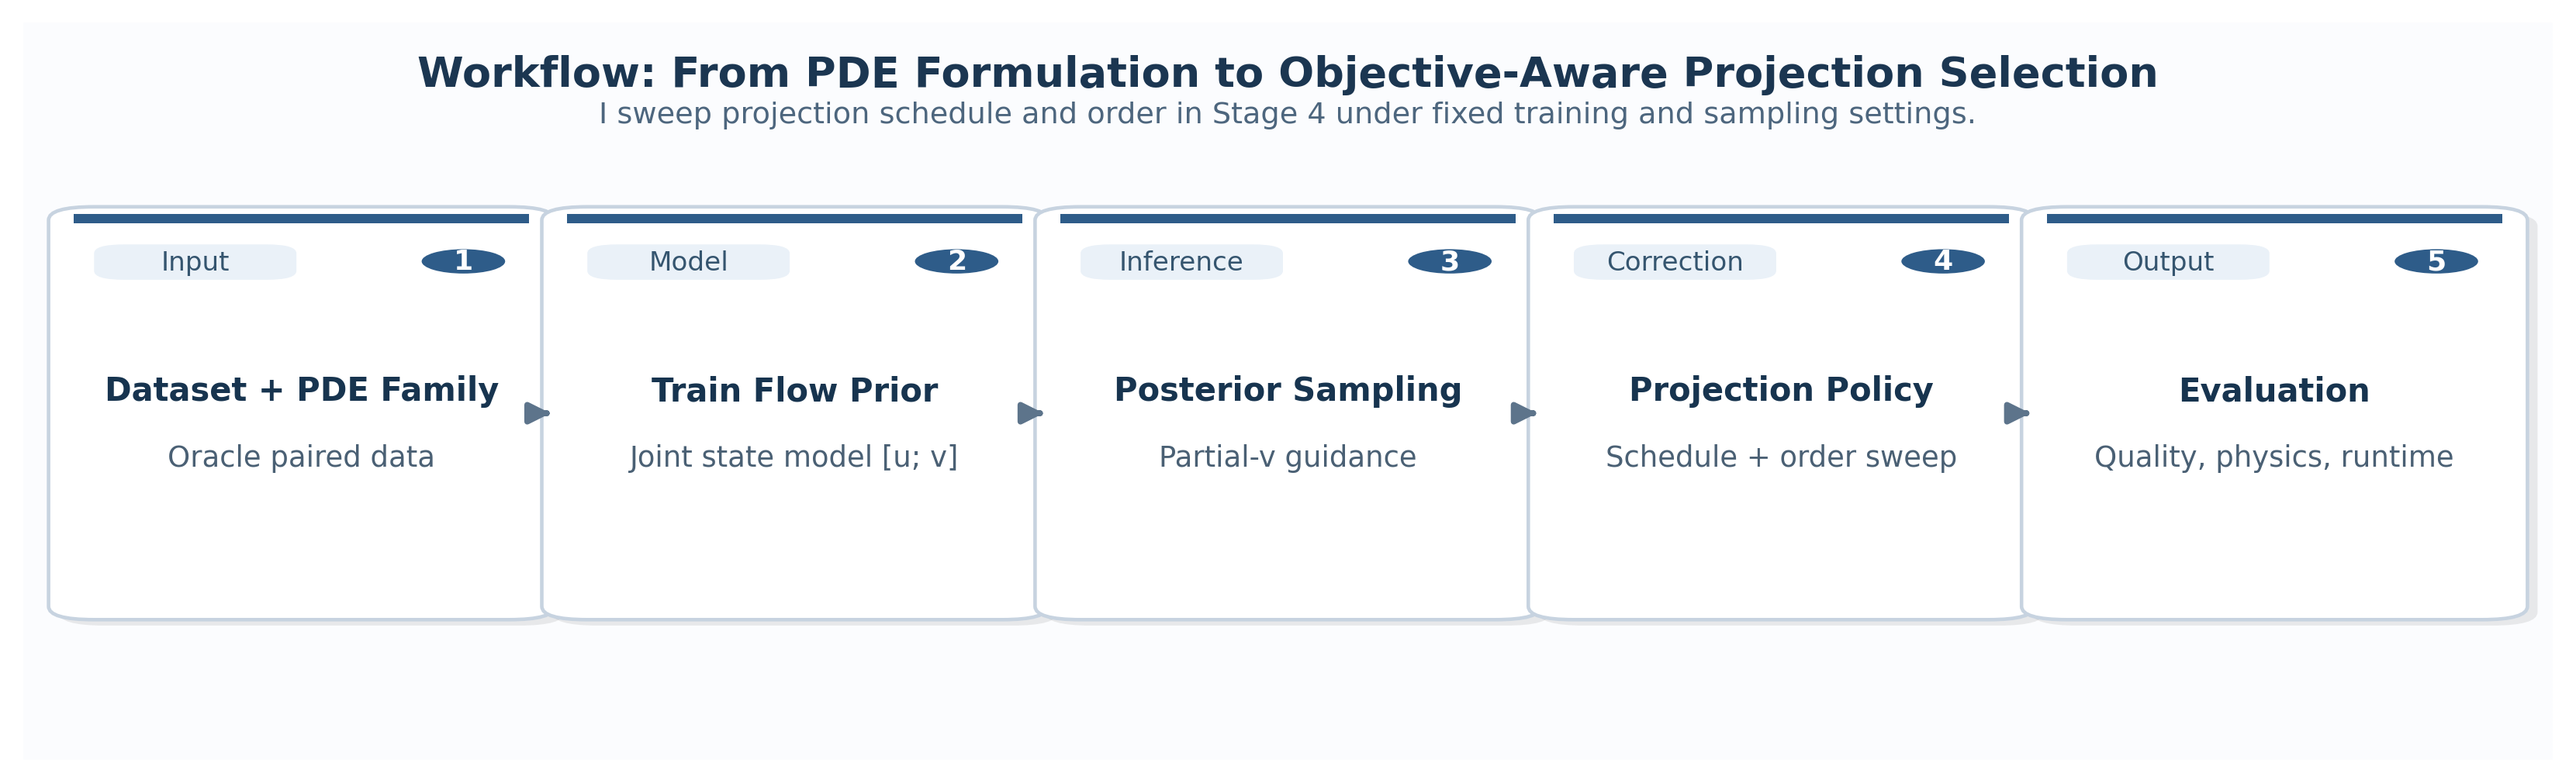
\includegraphics[width=0.90\textwidth]{workflow_flowchart.png}
\caption{Workflow from PDE-family data to objective-wise projection-policy selection. The schedule/order sweep is isolated while keeping inverse setup and evaluation logic fixed.}
\label{fig:workflow}
\end{figure*}

\section{Experimental Protocol}
Baseline uses the default 80-epoch checkpoint and default model width/depth. Tuned runs use stronger training and guidance sweeps, with the strongest nonlinear analysis at \(\texttt{e200\_big}\) and \(g=16\).

Nonlinear main-study evaluation uses 128 posterior samples and 3 observation seeds. Projection schedule candidates are
\texttt{none}, \texttt{final\_only}, \texttt{every\_step}, \texttt{every\_2}, \texttt{every\_5}, \texttt{late\_only}, and \texttt{adaptive\_residual}.

\begin{table}[h]
\centering
\small
\caption{Metric roles in this inverse setting.}
\begin{tabularx}{\columnwidth}{@{}lY@{}}
\toprule
\textbf{Metric} & \textbf{Interpretation} \\
\midrule
\texttt{u\_error} & Primary inverse-target accuracy \\
\texttt{v\_error} & Full-state reconstruction, incl.\ unobserved \(v\) \\
\texttt{obs\_error} & Fit quality on observed subset \\
\texttt{posterior\_quality} & Composite posterior-ranking score \\
\texttt{physical\_consistency} & Pre-cleanup PDE consistency \\
\texttt{runtime}, \texttt{trajectory\_stability} & Efficiency and numerical robustness \\
\texttt{mmse}, \texttt{smse}, \texttt{fpd} & Distribution-level metrics (pipeline support added) \\
\texttt{ce\_ic}, \texttt{ce\_bc}, \texttt{ce\_cl} & Family-specific constraint errors (N/A if not applicable) \\
\bottomrule
\end{tabularx}
\end{table}

\section{Results: Nonlinear Elliptic Benchmark}
\subsection{Objective-wise winners}
\begin{table*}[t]
\centering
\normalsize
\renewcommand{\arraystretch}{1.14}
\caption{Best schedule/order by objective (\(128\times3\) evaluation grid).}
\label{tab:obj_winners}
\begin{tabularx}{0.98\textwidth}{@{}lXl r@{}}
\toprule
\textbf{Objective} & \textbf{Winning run} & \textbf{Best policy} & \textbf{Value} \\
\midrule
\texttt{posterior\_quality} & \texttt{e200\_big} + strong guidance & \texttt{every\_5 / gauss\_newton} & 3.1364 \\
\texttt{physical\_consistency} & \texttt{e200\_big} + strong guidance & \texttt{every\_step / gauss\_newton} & 0.000359 \\
\texttt{runtime} & baseline checkpoint & \texttt{none / none} & 0.6086 s \\
\texttt{trajectory\_stability} & baseline checkpoint & \texttt{none / none} & 0.0 \\
\bottomrule
\end{tabularx}
\end{table*}

The winners are numerically distinct rather than tied, which confirms that projection policy should be selected per objective. A single global policy is suboptimal when deployment priorities differ.

\subsection{Best inverse row versus baseline}
\begin{table*}[t]
\centering
\normalsize
\caption{Best inverse row comparison (\(128\times3\)).}
\resizebox{0.93\textwidth}{!}{%
\begin{tabular}{@{}lccccc@{}}
\toprule
\textbf{Setting} & \(\mathbf{u\_err}\) & \(\mathbf{v\_err}\) & \(\mathbf{obs\_err}\) & \(\mathbf{post\_q}\) & \(\mathbf{runtime}\) \\
\midrule
Baseline best row & 1.9232 & 1.2944 & 1.1504 & 4.3679 & 0.7357 s \\
Best tuned row (\texttt{g=16}, \texttt{every\_step/first\_order}) & 1.5050 & 0.9120 & 0.8126 & 3.2295 & 1.3741 s \\
\midrule
Relative change & \(-21.75\%\) & \(-29.54\%\) & \(-29.36\%\) & \(-26.06\%\) & \(+86.77\%\) \\
\bottomrule
\end{tabular}%
}
\end{table*}

\textbf{Key result.} The strongest inverse-reconstruction configuration is \texttt{every\_step/first\_order} under strong guidance, with absolute improvements:\\
\(\mathbf{u\_error}: 1.9232\rightarrow 1.5050\),\\
\(\mathbf{v\_error}: 1.2944\rightarrow 0.9120\),\\
\(\mathbf{obs\_error}: 1.1504\rightarrow 0.8126\).

\begin{figure}[h]
\centering
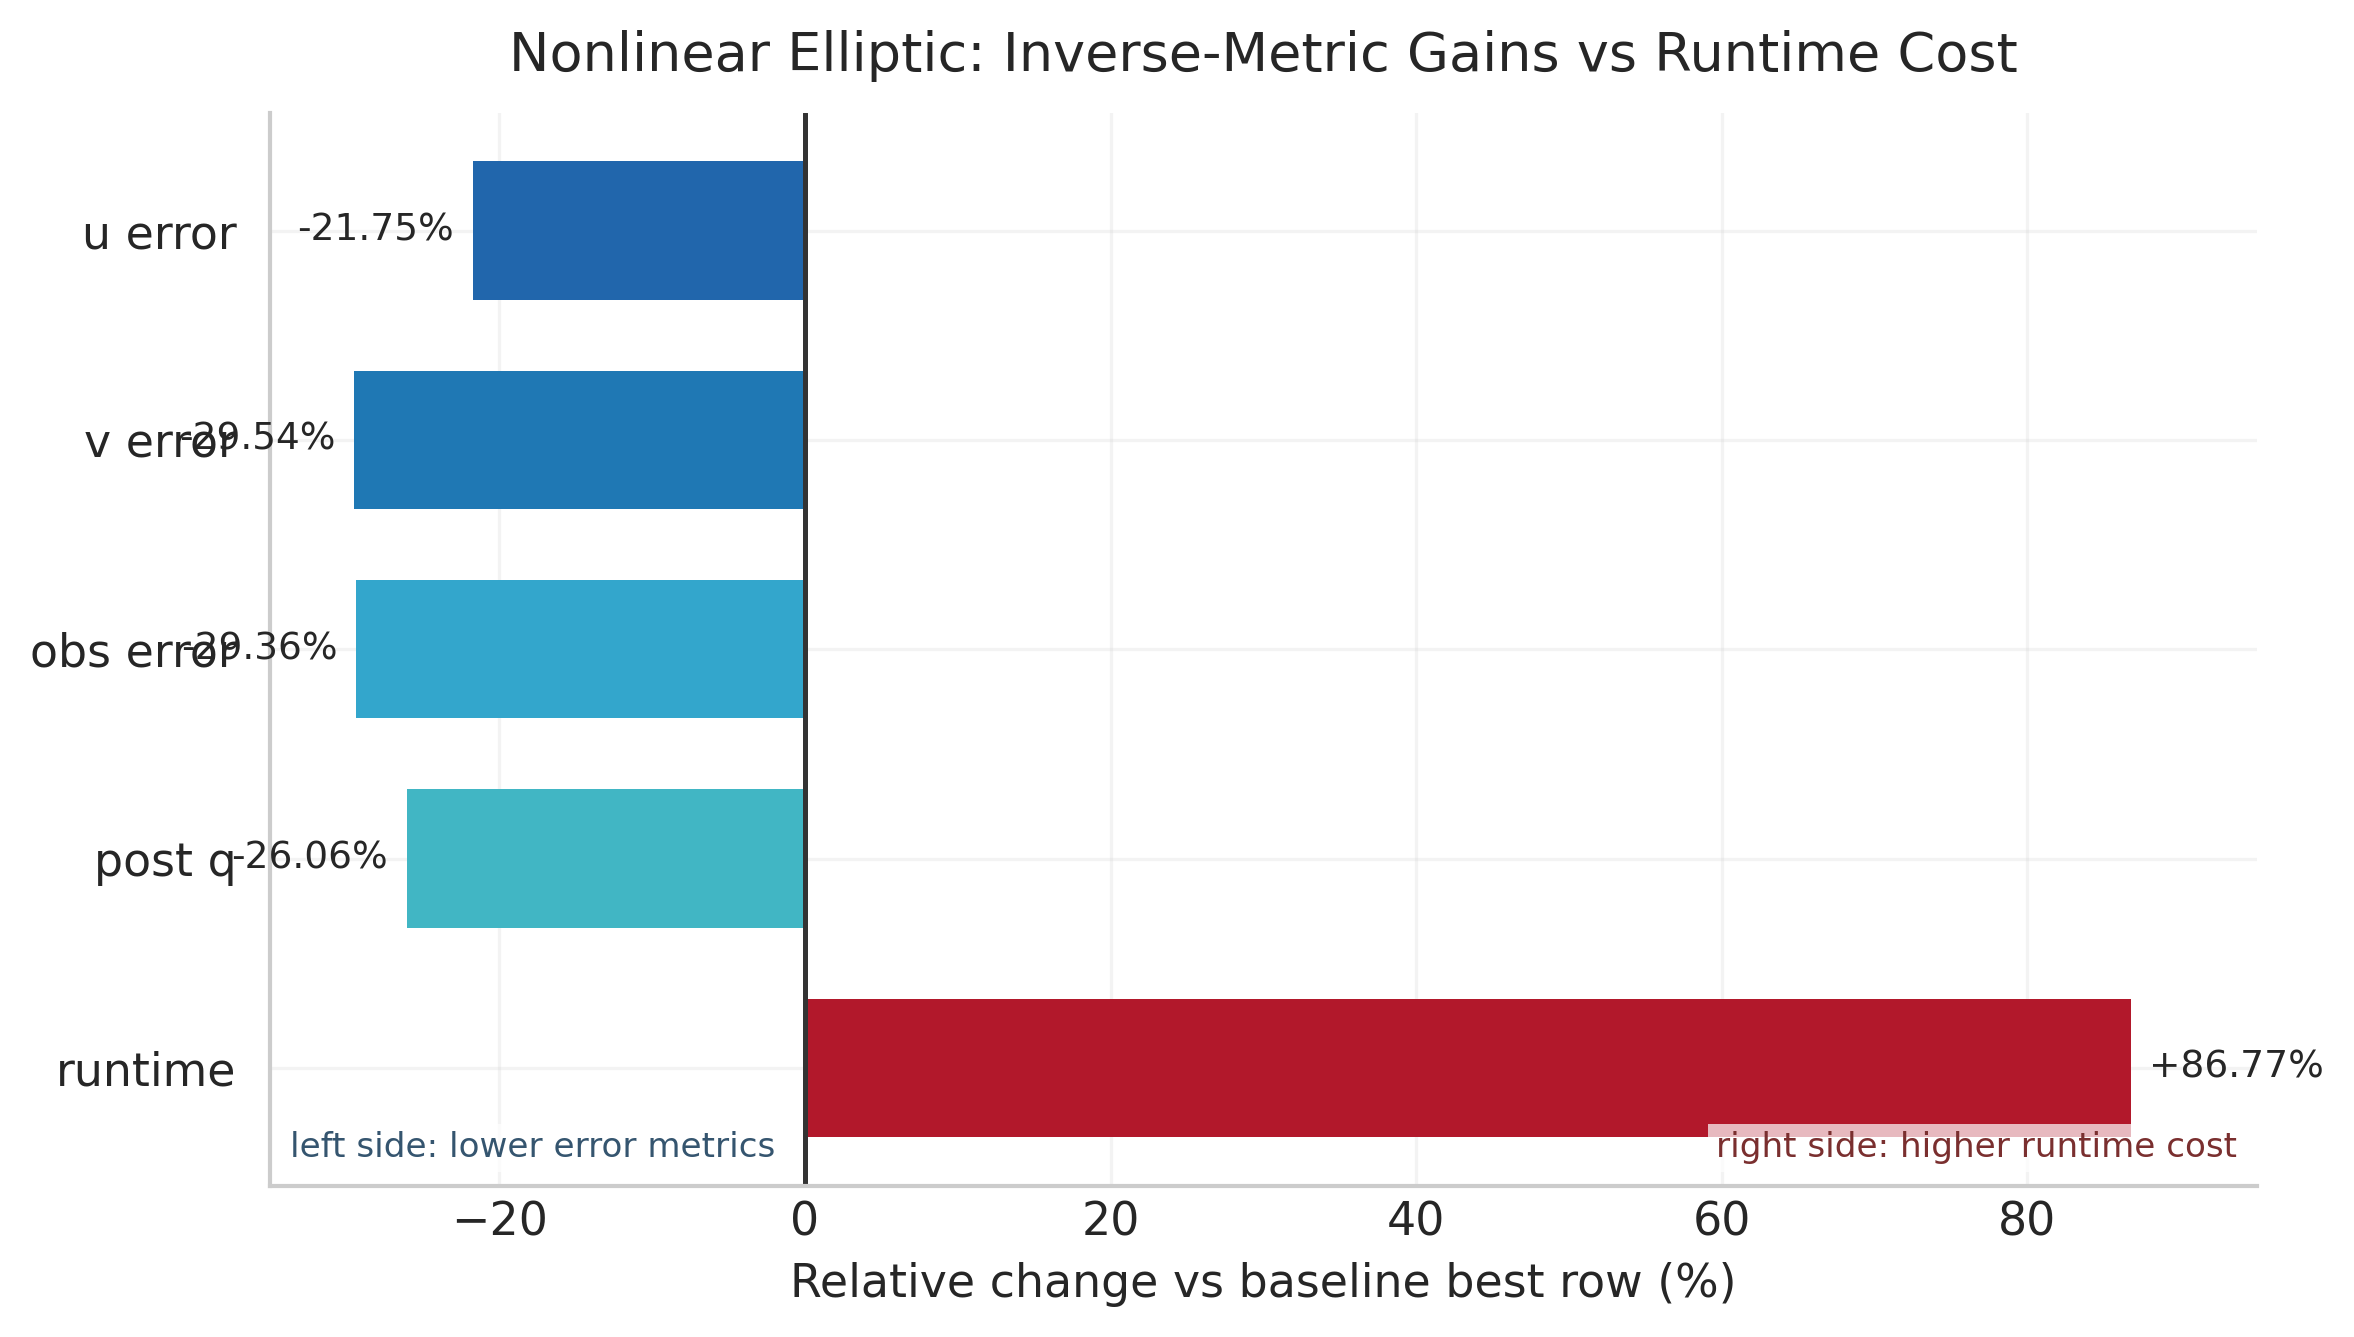
\includegraphics[width=\columnwidth]{nonlinear_gain_cost_scorecard.png}
\caption{Relative changes versus baseline for best inverse row. Error metrics decrease while runtime increases, quantifying the gain-cost tradeoff directly.}
\label{fig:gaincost}
\end{figure}

\begin{figure}[h]
\centering
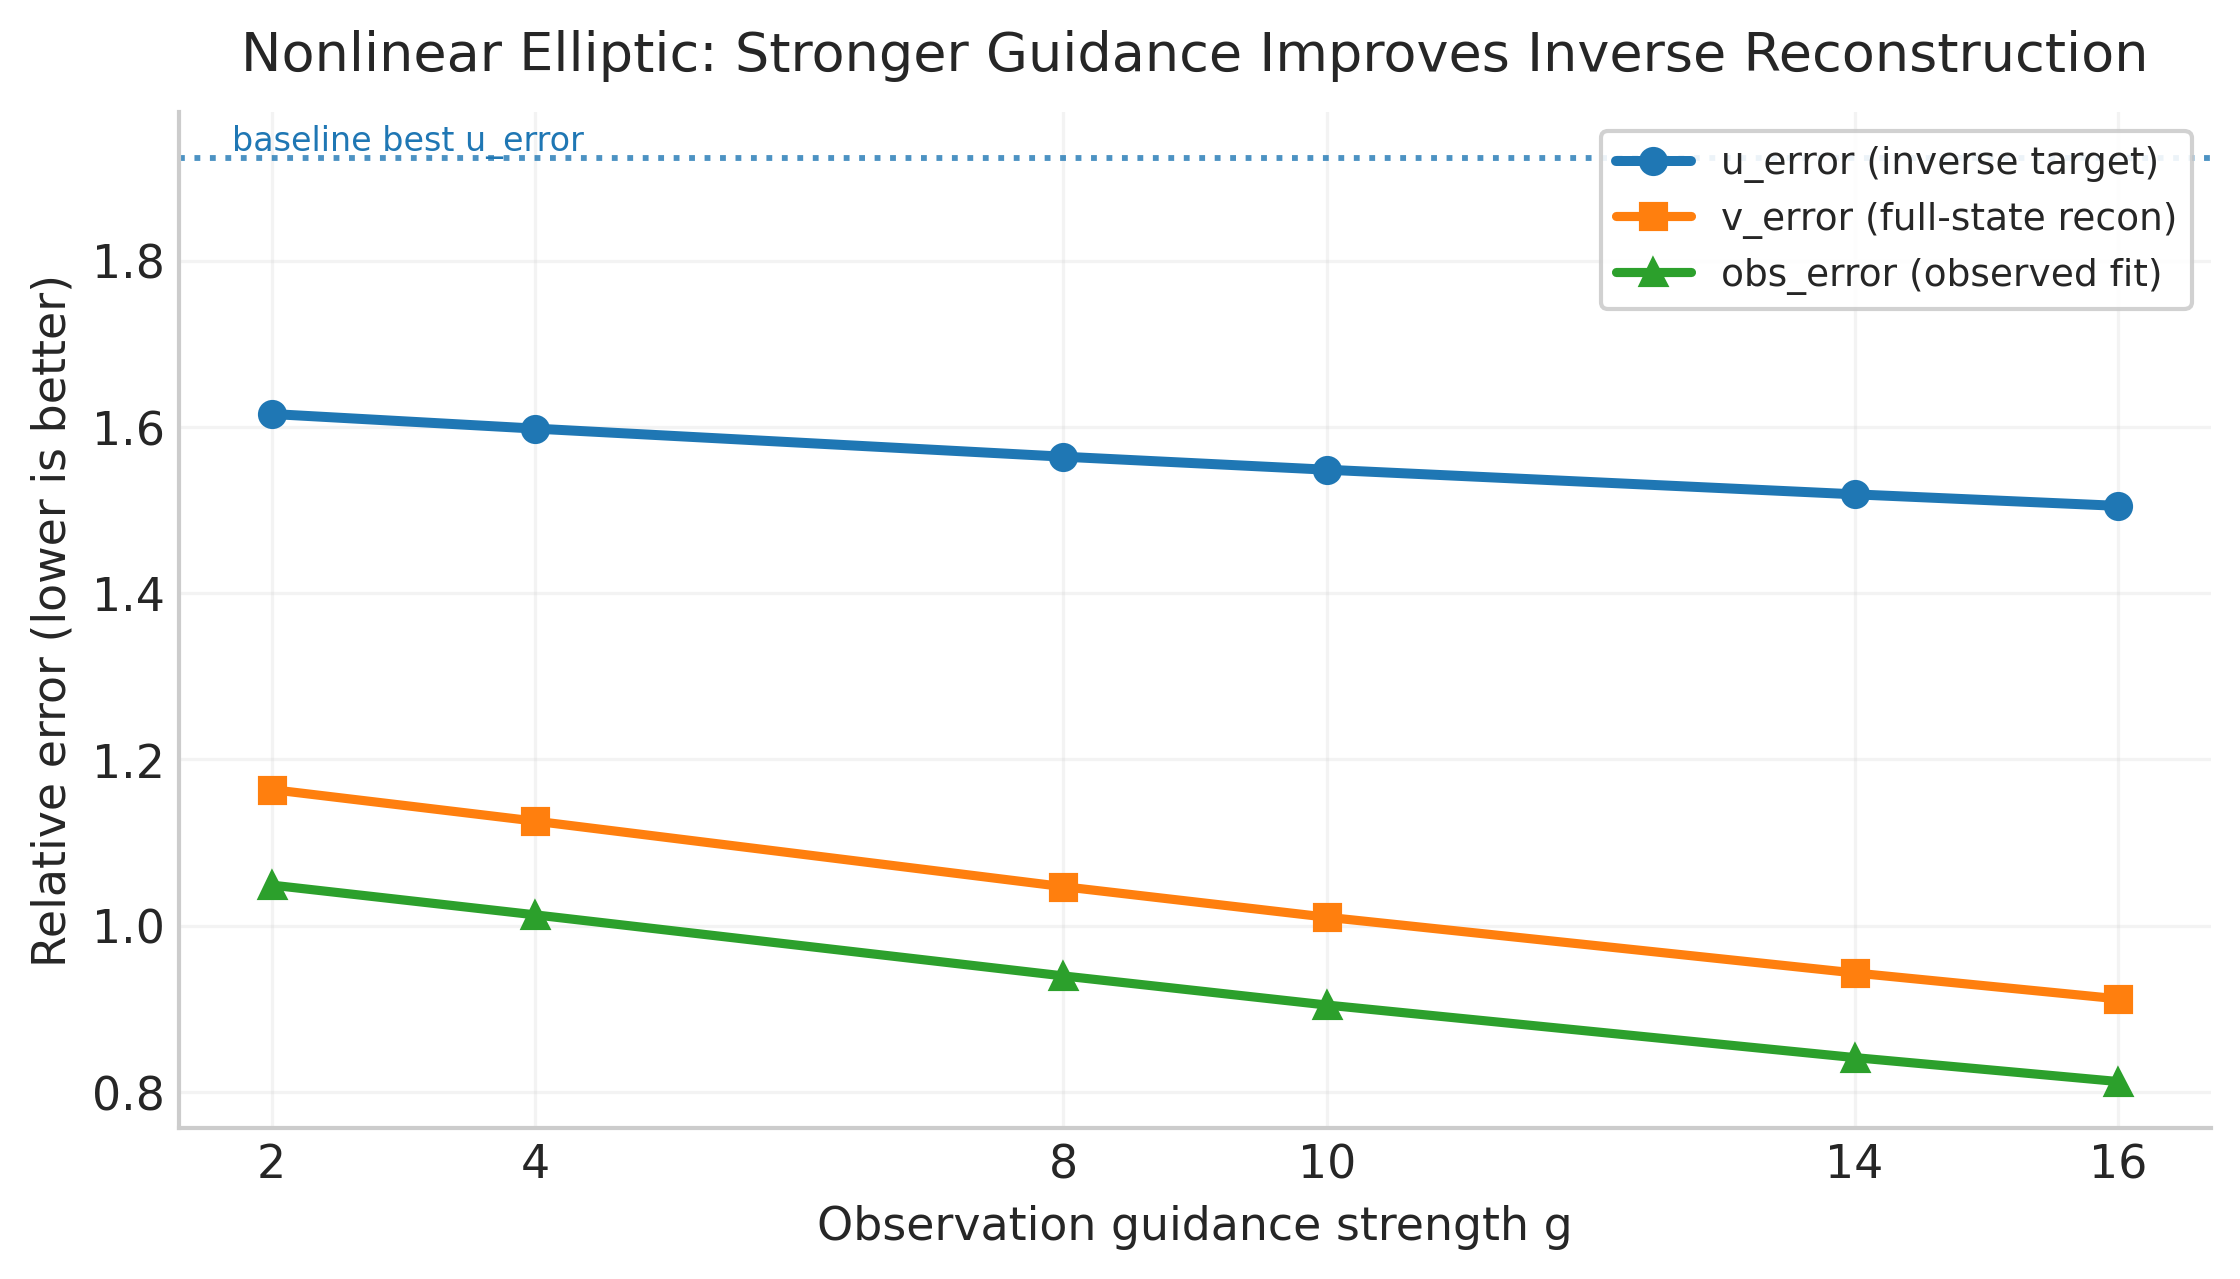
\includegraphics[width=\columnwidth]{nonlinear_guidance_trend.png}
\caption{Guidance sweep on nonlinear elliptic benchmark. Higher guidance consistently improves inverse reconstruction metrics.}
\label{fig:guidance}
\end{figure}

\begin{figure*}[t]
\centering
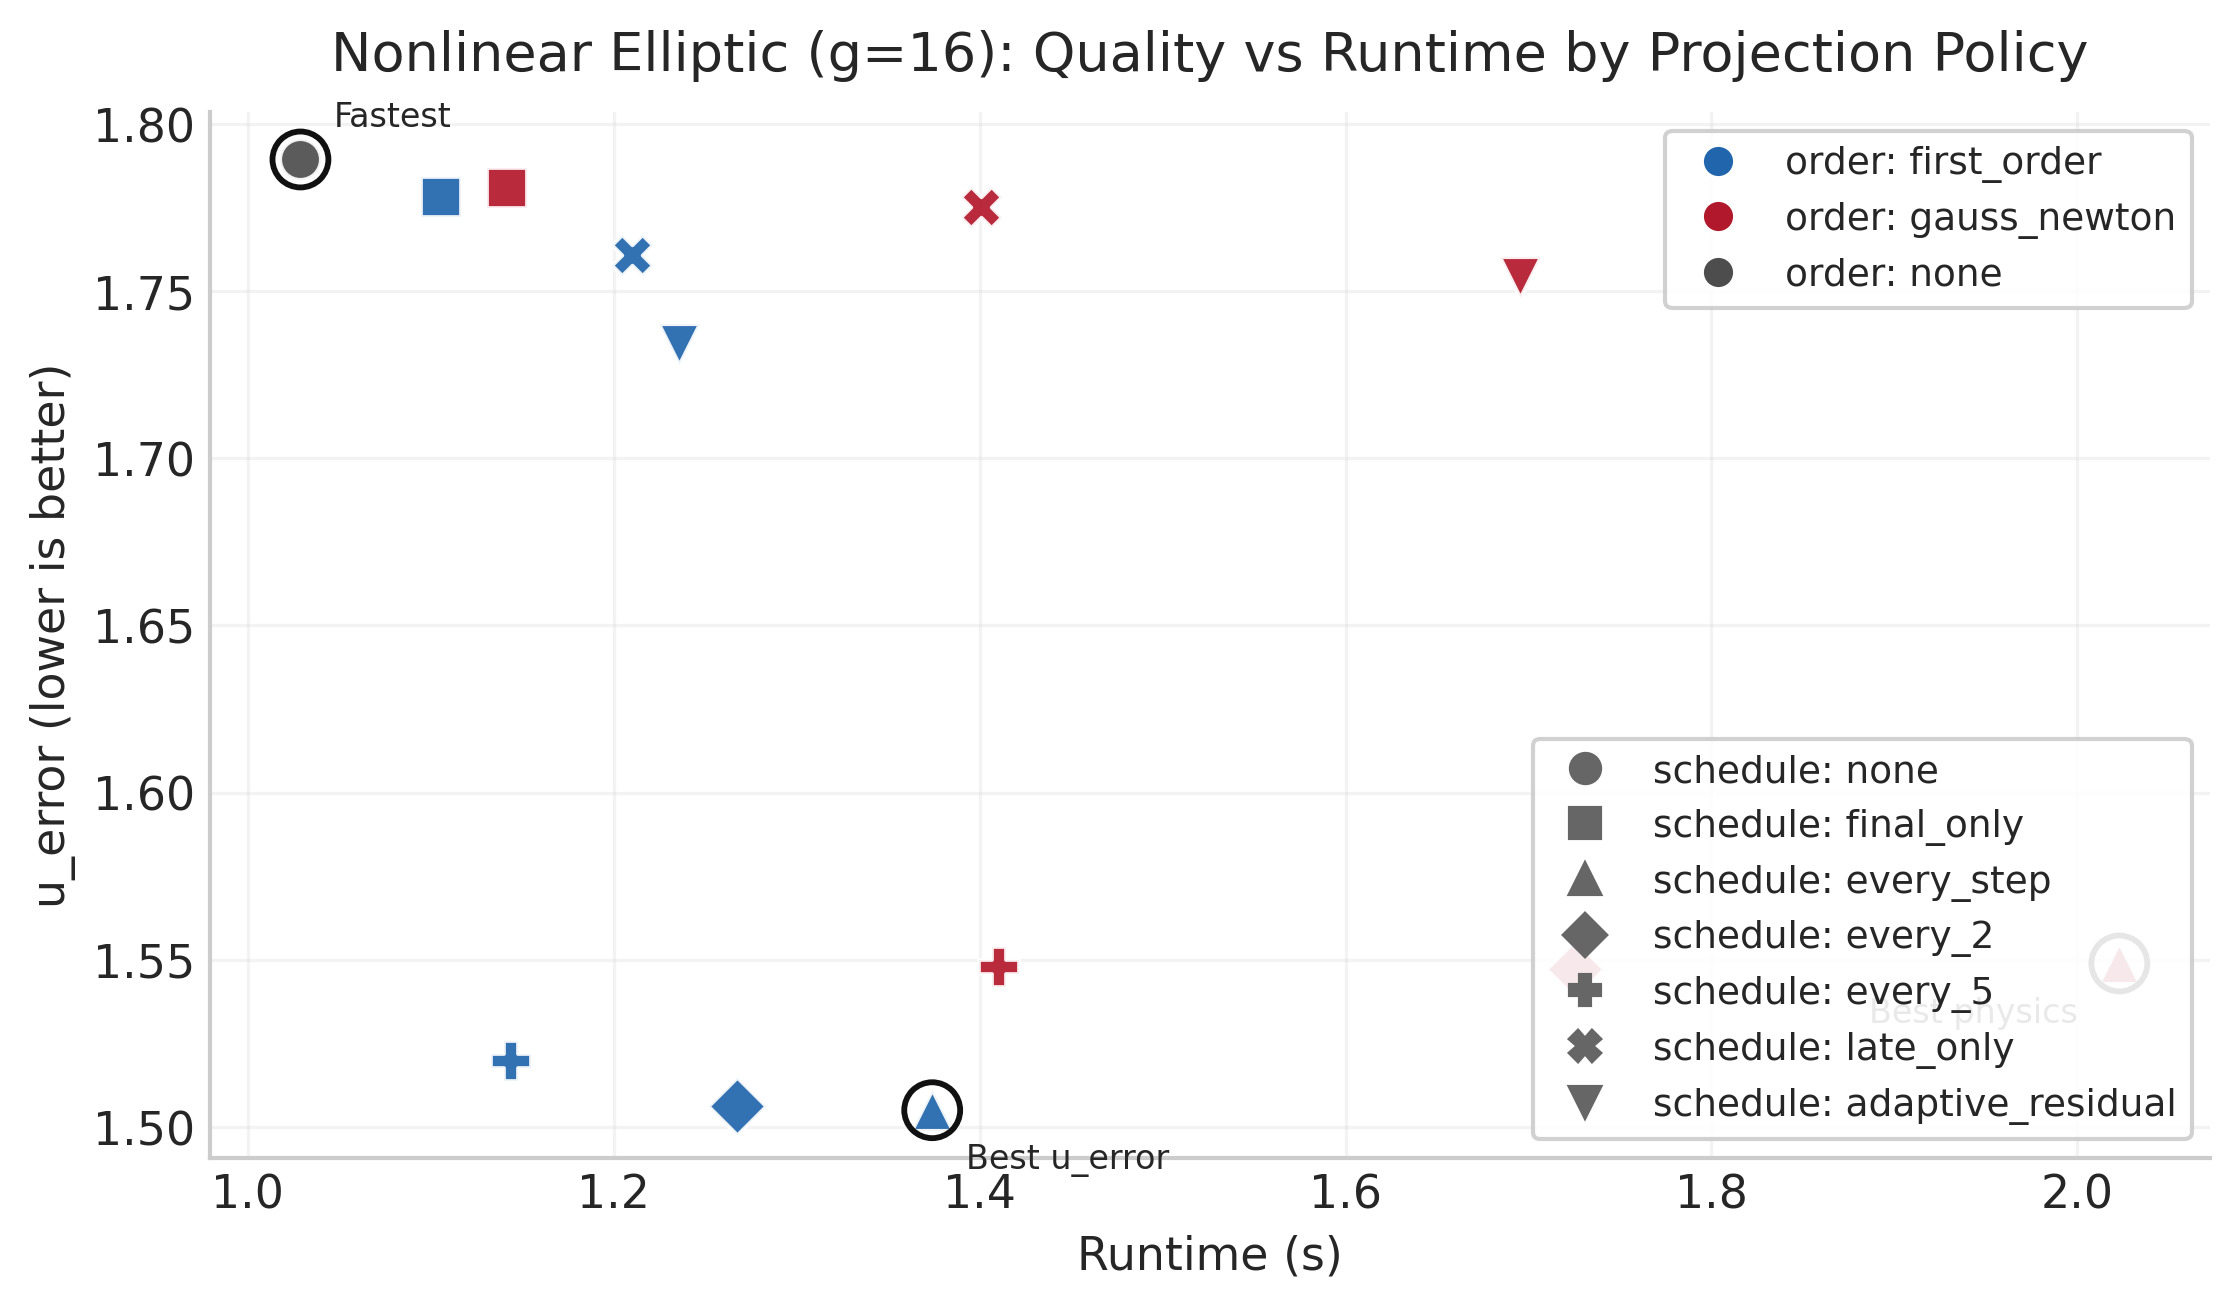
\includegraphics[width=0.76\textwidth]{nonlinear_tradeoff_scatter.png}
\caption{Quality-runtime frontier at \(g=16\). Marker shape indicates schedule, color indicates projection order.}
\label{fig:tradeoff}
\end{figure*}

\section{Results: Multi-Family Extension}
The same evaluation protocol is applied to linear elliptic, heat equation, reaction-diffusion, Burgers (IC/BC), and a 1D Navier-Stokes surrogate.

\begin{table}[h]
\centering
\small
\caption{Best-row \(u\_error\) change from \(g=0.25\) to \(g=16\).}
\begin{tabular}{@{}lr@{}}
\toprule
\textbf{Family} & \textbf{\(u\_error\) reduction} \\
\midrule
Linear elliptic & \(-18.73\%\) \\
Heat equation & \(-25.20\%\) \\
Reaction-diffusion & \(-29.84\%\) \\
Burgers IC & \(-26.12\%\) \\
Burgers BC & \(-9.03\%\) \\
Navier-Stokes 1D surrogate & \(-24.11\%\) \\
\bottomrule
\end{tabular}
\end{table}

\begin{figure}[h]
\centering
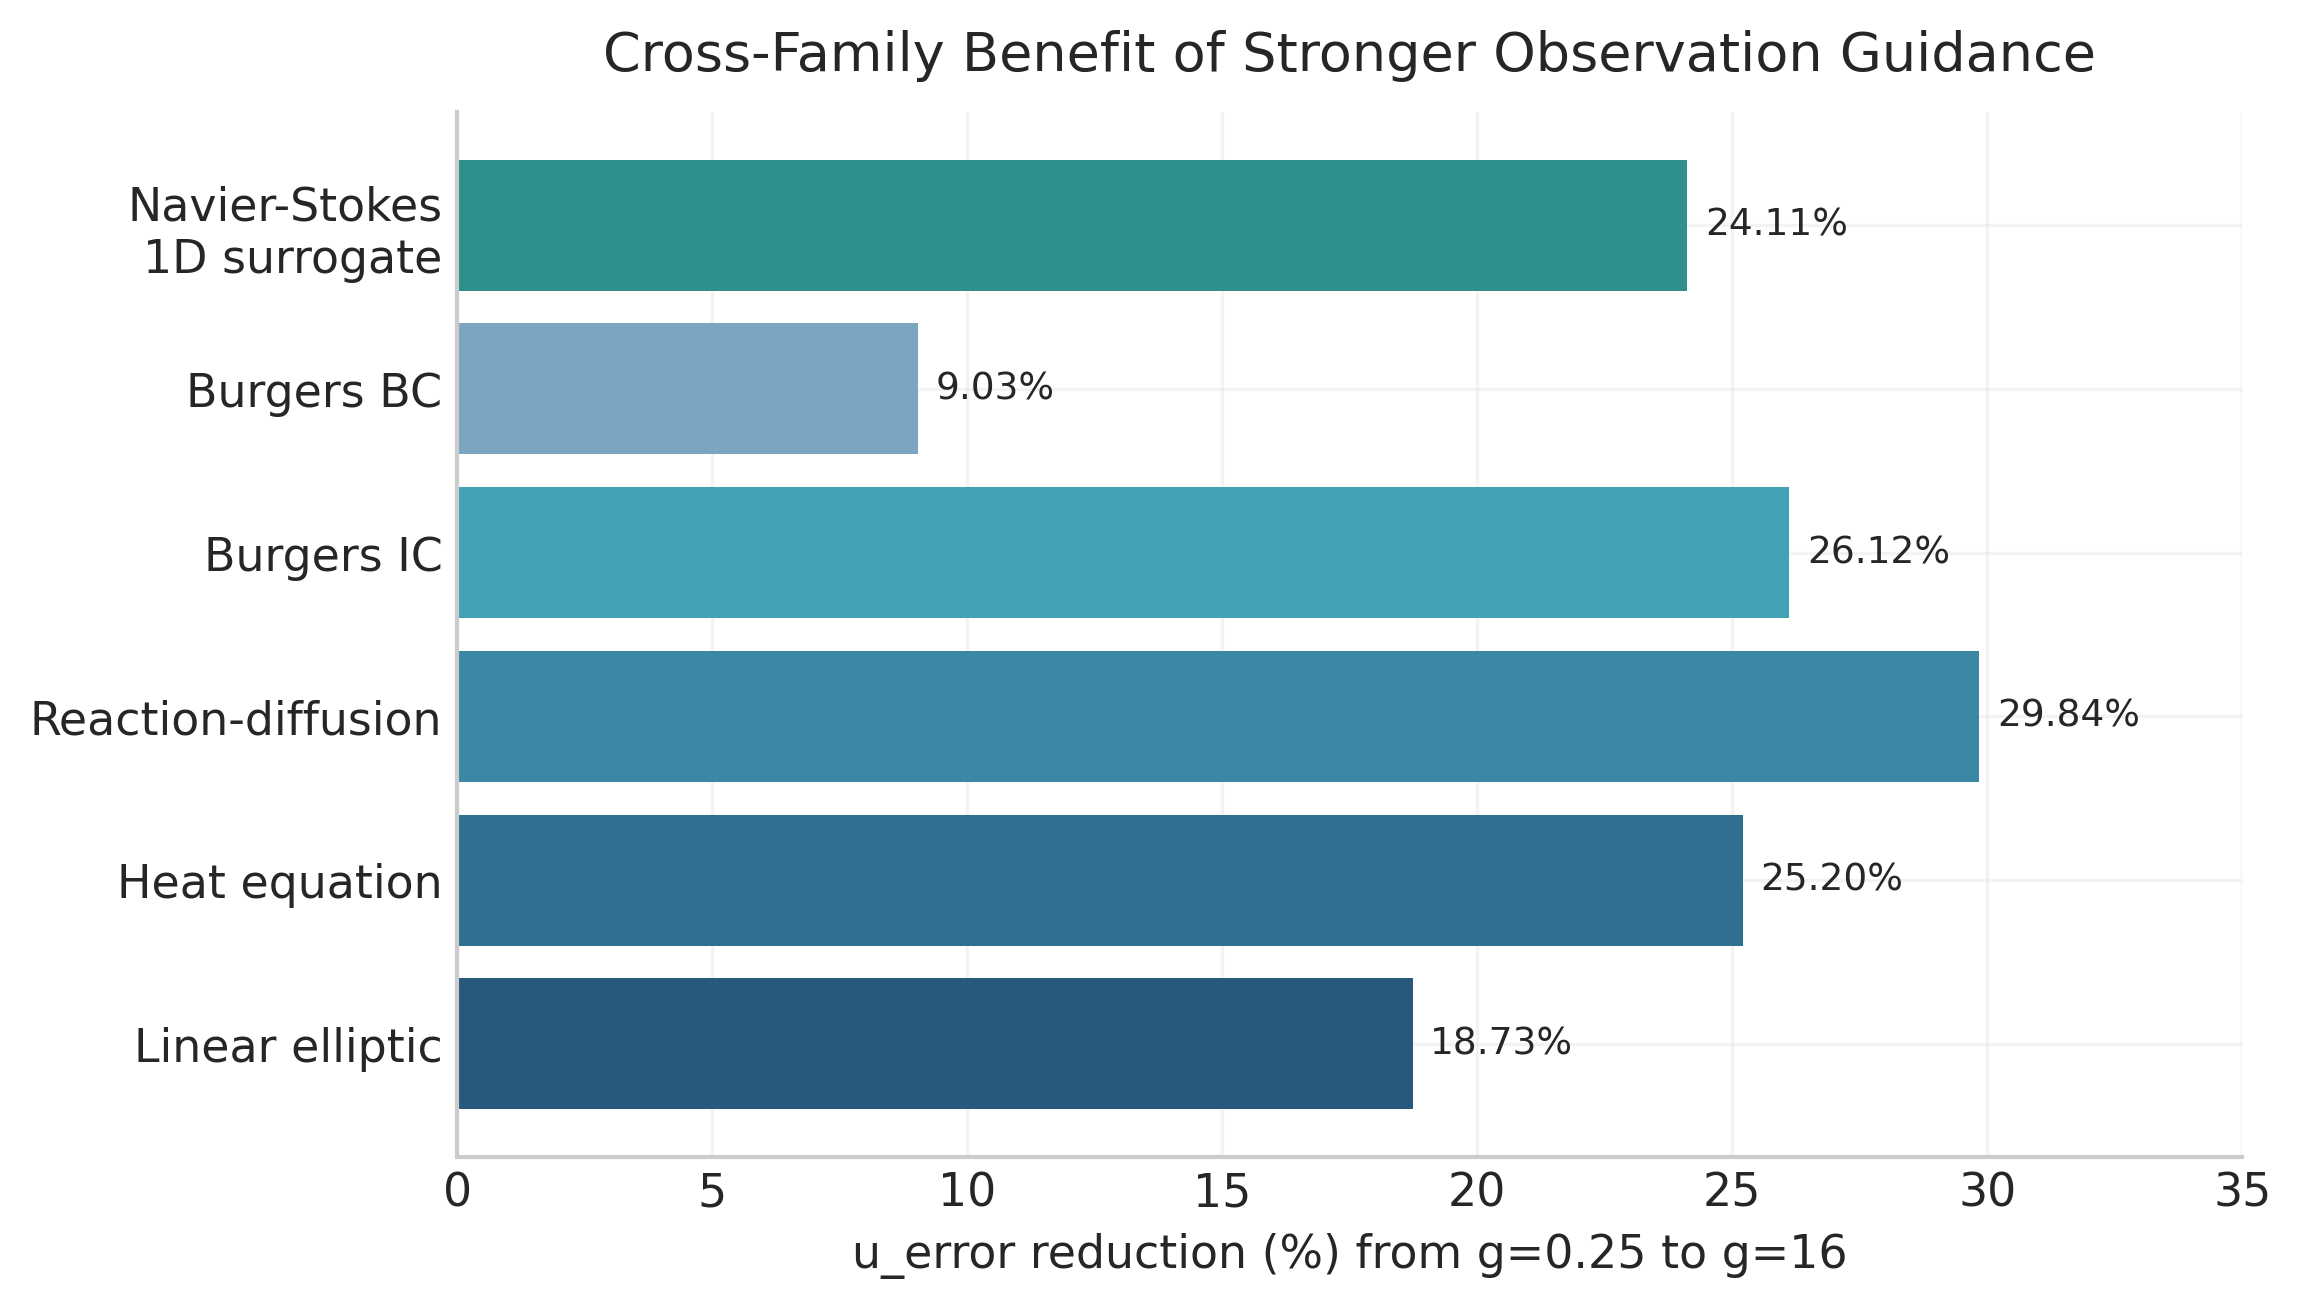
\includegraphics[width=\columnwidth]{cross_family_u_improvement.png}
\caption{Cross-family inverse-recovery gains from stronger guidance.}
\label{fig:crossfamily}
\end{figure}

\textbf{Interpretation.} Stronger guidance helps every tested family, with gains ranging from \(-9.03\%\) to \(-29.84\%\), supporting the robustness of guidance tuning beyond one PDE type.

\section{Discussion}
Three practical conclusions follow from the results.
\begin{itemize}
  \item For best inverse reconstruction, strong guidance with frequent first-order projection is most effective (\(u\_error=1.5050\), \(v\_error=0.9120\)).
  \item For strongest physical consistency, Gauss-Newton projection at every step performs best (\(0.000359\)).
  \item For strict runtime/stability budgets, no projection remains preferred (\(0.6086\) s, \(\texttt{trajectory\_stability}=0.0\)).
\end{itemize}
This objective-dependent pattern matches PCFM intuition \cite{pcfm}: projection is a control mechanism, and the correction policy should be tuned to the deployment target rather than fixed a priori.

\section{Limitations and Reproducibility}
The study intentionally prioritizes interpretability and reproducibility over exhaustive benchmarking. Full cross-method reproduction of all published baselines is outside scope. Nonetheless, all experiments are script-driven, metric definitions are explicit, and artifacts are tracked in the repository \cite{repo}.

Existing backend components in \texttt{src/chonkdiff} are reused for oracle/benchmark generation, while posterior-projection implementation and sweeps are implemented in \texttt{src/posterior\_projection}. LLM assistance was used for coding and drafting, and all reported metrics were manually verified.

\section{Conclusion}
Projection schedule and order are first-class design choices in partial-observation inverse PDE sampling. On the nonlinear benchmark, the best inverse policy improves \(u\_error\) by \(21.75\%\) and \(v\_error\) by \(29.54\%\), while best physics and best runtime are attained by different policies. The central implication is methodological: projection should be treated as an objective-aware policy variable, not a fixed post-processing step.

\begin{thebibliography}{9}
\bibitem{diffusionpde}
J. Huang, G. Yang, Z. Wang, and J. J. Park, \href{https://proceedings.neurips.cc/paper_files/paper/2024/hash/eb3878c1dcbfff9ee95d5d033e5f5942-Abstract-Conference.html}{\emph{DiffusionPDE: Generative PDE-Solving Under Partial Observation}}, NeurIPS 2024.

\bibitem{pcfm}
U. Utkarsh, P. Cai, A. Edelman, R. Gomez-Bombarelli, and C. V. Rackauckas, \href{https://arxiv.org/abs/2506.04171}{\emph{Physics-Constrained Flow Matching: Sampling Generative Models with Hard Constraints}}, 2025.

\bibitem{flowmatching}
Y. Lipman, R. T. Q. Chen, H. Ben-Hamu, M. Nickel, and M. Le, \href{https://arxiv.org/abs/2210.02747}{\emph{Flow Matching for Generative Modeling}}, ICLR 2023.

\bibitem{pcfmcode}
P. Cai and collaborators, \href{https://github.com/cpfpengfei/PCFM}{\emph{Physics-Constrained Flow Matching: code repository}}.

\bibitem{repo}
H. Zhu and collaborators, \href{https://github.com/hanshengzhu0001/meam4600_final_proj}{\emph{MEAM4600 Final Project Repository: Posterior Projection for PDE Generative Sampling}}.
\end{thebibliography}

\end{document}
